\documentclass{article}
\usepackage{mathtools}
\usepackage{caption}
\usepackage{subcaption}
\usepackage{enumitem}
\usepackage{multicol}
\usepackage[toc,page]{appendix}
\usepackage[gen]{eurosym}
\usepackage{tabularx}
\usepackage{epigraph}
\usepackage{textcomp}
\usepackage[english]{babel}
\usepackage[utf8]{inputenc}
\usepackage{amsmath}
\usepackage{amsthm}
\usepackage{amssymb}
\usepackage{hyperref}
\usepackage{csquotes}% Recommended
\usepackage{rotating}
\usepackage[style=numeric]{biblatex}
% \bibliography{<mybibfile>}% ONLY selects .bib file; syntax for version <= 1.1b
\addbibresource{literature.bib}% Syntax for version >= 1.2

\usepackage{graphicx}
\graphicspath{{./images/}}

\usepackage{fancyhdr}
\pagestyle{fancy}
\lhead{}
\chead{}
\rhead{}
\lfoot{}
\cfoot{\thepage}
\rfoot{Property of V-Research S.r.l.}
\renewcommand\headrulewidth{0pt}
\renewcommand\footrulewidth{0pt}

\usepackage[colorinlistoftodos]{todonotes}

\newcommand{\Paragraph}[1]{\smallskip\noindent{\bf #1.}}
\newcommand{\fixnote}[2]{\textbf{\color{red}{FIX}}\footnote{{\bf #1:} #2}}
\newcommand{\fix}[2]{{\color{red} {\bf tofix:} #2}}
% \renewcommand{\fixnote}[2]{}
% \renewcommand{\fix}[2]{}

\theoremstyle{definition}
\newtheorem{definition}{Definition}[section]
\theoremstyle{corollary}
\newtheorem{corollary}{Corollary}[section]
\theoremstyle{lemma}
\newtheorem{lemma}{Lemma}[section]
\theoremstyle{theorem}
\newtheorem{theorem}{Theorem}[section]
\theoremstyle{theorem}
\newtheorem{example}{Example}

\usepackage{authblk}
\date{}                     %% if you don't need date to appear
\setcounter{Maxaffil}{0}
\renewcommand\Affilfont{\itshape\small}

% for fancy table with rotated column titles
\usepackage{adjustbox}
\newcolumntype{R}[2]{%
    >{\adjustbox{angle=#1,lap=\width-(#2)}\bgroup}%
    l%
    <{\egroup}%
}
\newcommand*\rot{\multicolumn{1}{R{45}{0.01em}}}% no optional argument here, please!
\newcommand*\rota{\multicolumn{1}{R{90}{0.01em}}}% no optional argument here, please!
\def\hb{\hbox to 10.7 cm{}}

% circles
\usepackage{wasysym}
\newcommand{\Tdot}{$\CIRCLE$}
\newcommand{\Thdot}{$\LEFTcircle$}
\newcommand{\Twdot}{$\Circle$}

% formulas
\newcommand{\kframe}{\mathbf{K}}
\newcommand{\bframe}{\mathbf{B_K}}
\newcommand{\possibleworlds}{G}
\newcommand{\modalrelation}{R}
\newcommand{\actualworld}{\omega*}
\newcommand{\world}{\omega}
\newcommand{\World}{\Omega}
\newcommand{\kmodel}{M}
\newcommand{\interpretation}{\sigma}
\newcommand{\knowledge}[1]{\mathbb{K}_{#1}}
\newcommand{\knows}[2]{K_{#1}#2}
\newcommand{\belief}[1]{\mathbb{B}_{#1}}
\newcommand{\believe}[2]{B_{#1}#2}
\newcommand{\region}{\chi}
\newcommand{\Region}{\mathrm{X}}
\newcommand{\agentuniverse}{\mathcal{A}}
\newcommand{\agent}{a}
\newcommand{\follang}{\mathcal{L}}
\newcommand{\weakness}{w}
\newcommand{\Weakness}{W}
\newcommand{\vulnerability}{v}
\newcommand{\Vulnerability}{V}
%rcc5
\newcommand{\rcc}{rcc}
\newcommand{\connects}[2]{C(#1,#2)}
\newcommand{\disconnected}[2]{\neg C(#1,#2)}
\newcommand{\partof}[2]{P(#1,#2)}
\newcommand{\overlaps}[2]{O(#1,#2)}
\newcommand{\eq}[2]{EQ(#1,#2)}
\newcommand{\pp}[2]{PP(#1,#2)}
\newcommand{\po}[2]{PO(#1,#2)}
\newcommand{\ppi}[2]{PPi(#1,#2)}
\newcommand{\dr}[2]{DR(#1,#2)}


\makeindex 

\begin{document}

\title{On Cybersecurity\\Science and Engineering\footnote{Confidential, restricted to the authors. Property of V-Research S.r.l.}}
\author[1]{Francesco Beltramini}
\author[1]{Marco Rocchetto}
\author[2]{Luca Vigan\`o}
\affil[1]{V-Research, Verona, Italy}
\affil[2]{King's College London, UK}

\maketitle

\begin{abstract}
	The objective of this research is to develop of a theory that defines
	(all and only) the possible insecurity and security configurations of
	any abstract system. The theory is structured upon other theories that 
	defines how a component of a system can be abstracted into an agent, defining how
	agents can be formalized (both syntactically and semantically) to
	describe an abstract system, such as a graph. Some of these theories
	(e.g. used for the semantic
	definition of the abstract system) are the epistemological definition
	of knowledge, the Belief-Desire-Intent and the Assertion-Belief-Fact 
	framework of reference, 
	mereology, and topological structure. We argue that a mereology is the
	most appropriate abstract underlying structure, do to its generality,
	for defining the expressiveness of the system abstraction.  Furthermore, a
	mereology allows us to define an ontology rather than a taxonomy.  We
	also correlate different abstractions of the system to the TRL and the
	engineering V-model. 
	
	We implemented a formal theory (of axioms) of a mereotopology, and of
	the Region Connection Calculus (RCC3 and RCC5) in a Python program that
	uses the Z3 SMT solver. The results show that a single component (i.e.
	agent) of an abstract system has a definite number of  different
	insecurity configurations (e.g. 53 using RCC5 over a topological
	structure) and only 1 secure (i.e. expected) configurations. The
	configurations are reported as models satisfying the abstract system
	semantics. 
	
	We considered the philosophical definition of truth behind our
	approach, rejecting ``proof'' by induction from partial empirical evidences.
	Our theory can be applied to system engineering and we show a concrete
	application of our theory to the risk assessment of an ad-hoc system.
	Finally, we provide a number of ideas to support the engineering of
	secure systems (e.g. purely cyber or cyber-physical).
\end{abstract}
\newpage

\section{Introduction}\label{sec:intro}
\epigraph{Humanum est errare}{{\itshape Seneca the Elder}}
The European Commission states in\autocite{EU2019market} that: ``Cybersecurity
is one of the priority areas [\ldots] of the Commission initiative on ICT
Standards, which is part of the Digitising European
Industry\autocite{EU2019standard} strategy launched on 19 April 2016.  The aim
is to identify the essential ICT standards and present measures to accelerate
their development in support of digital innovations across the economy''. The
same document (i.e.\autocite{EU2019market}) states that ``The EU will invest up
to \euro450 million [\ldots], under its research and innovation programme
Horizon 2020''. The EU, in 2016 published a press release\autocite{EU2016press}
in which they present a strategy to invest \euro1.8 \emph{billion} to
``increase measures to address cyber threats''. The EU is not the only investor
in cybersecurity, most of the developed countries and several companies are
investing enormous amount of money towards various aspects of cybersecurity
(e.g. The US vulnerability databases\autocite{NIST2020NVD} maintained by the
National Institute of Standards and Technologies, i.e. NIST, of the US
Department of Commerce).

The cybersecurity industry is growing fast, e.g. as reported
in\autocite{Nasdaq2018market}. For example, in\autocite{Forbes2017market},
published by the Forbes, is stated that \euro5.3 billion of funding where
poured by venture capitalist into cybersecurity companies in 2018. The Forbes,
in the same article, also highlights another peculiar (as seemly contradictory)
trend: ``[\ldots] during the same time period, the number of cybersecurity
breaches increased exponentially''. The data reported by the NIST 
through the official CPE (Common Platform Enumeration) Dictionary Statistics 
on the NVD websites in \autocite{NIST2020CPEstatistics}, show that in 2016 the
number of reported vulnerabilities reported where around $~6000$ while in 2019
the number of vulnerabilities was above $16000$.  The scientific community also
reports similar findings.  In fact, in\autocite{Herley2009so}, Cormac Herley
(Microsoft Research) shows how basic cybersecurity principles (such as the
confidentiality benefit over the clear text for passwords typed into forms,
e.g. for logins in websites) are not fully understood or shared between the
cybersecurity research community\autocite{Nielsen2009stop}.  The lack of
understanding of basic security principle, the inverse proportionality between
investments in cybersecurity and the number of reported vulnerabilities year
after year, can be linked to the lack of a foundational theory on
cybersecurity, as already highlighted by Cormac Herley
in\autocite{Herley2016unfalsifiability}. 

Another way of looking at the same problem is by analyzing the different
definitions of security with respect to the scientific method of enquiry
applied to get to the definition itself. In the following we categorize the
related work into three categories, as defined by Sextus Empiricus in
\autocite{Empiricus1990Pyrrhonism}.  To the best of our knowledge, there is no
evidence that this categorization isn't complete.  ``The natural result of any
investigation is that the investigators either discover the object of search or
deny that it is discoverable and confess it to be in-apprehensible or persist
in their search. [\ldots] This is probably
why''\autocite{Empiricus1990Pyrrhonism}: 
\begin{itemize}
	\item The \emph{dogmatists} ``have claimed to have discovered the truth'' on what cybersecurity is
		\begin{itemize}
			\item Wikipedia defines cybersecurity in
				\autocite{wiki-cybersecurity} as the protection
				of computer systems and networks from the theft
				of or damage to their hardware, software, or
				electronic data, as well as from the disruption
				or misdirection of the services they provide
		\end{itemize}
	\item The \emph{academics} ``have asserted that it cannot be apprehended''
		\begin{itemize}
			\item Eugene H. Spafford, Professor at Purdue
				University, defines cybersecurity as follow.
				``The only truly secure system is one that is
				powered off, cast in a block of concrete and
				sealed in a lead-lined room with armed guards —
				and even then I have my doubts.''
				\autocite{Spafford2019Quotes}
		\end{itemize}
	\item The \emph{skeptics} ``go on inquiring''
		\begin{itemize}
			\item Cormac Herley reaches the conclusion that
				cybersecurity has no definition. ``There is an
				inherent asymmetry in computer security: things
				can be declared insecure by observation, but
				not the reverse. There is no test that allows
				us to declare an arbitrary system or technique
				secure. This implies that claims of necessary
				conditions for security are unfalsifiable. ''
				\autocite{Herley2016unfalsifiability}
		\end{itemize}
\end{itemize}

In this article, we give the first scientific theory (to the best of our knowledge)
on security.

\Paragraph{Structure} In Section~\ref{sec:problem} we define and formalize the problem statement. 
In Section~\ref{sec:theory} we outline our security theory, and in Section~\ref{sec:prototest}
we describe the implementation of the theory and some empirical tests of the theory.
Finally, in Section~\ref{sec:related} we conclude the paper with an overview of the related work.


\section{Problem Statement}\label{sec:problem}

\begin{figure}[t]
	\centering
	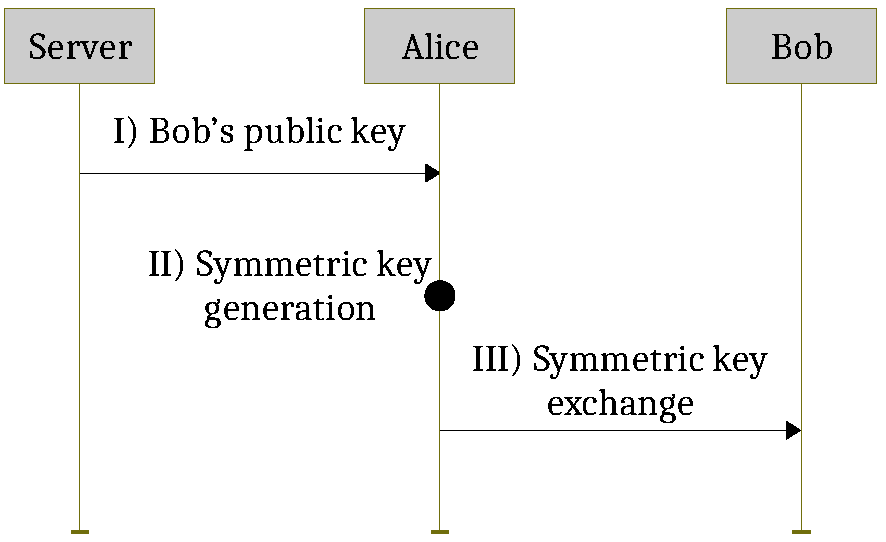
\includegraphics[width=.6\textwidth]{protocol-example.pdf}
	\caption{Abstraction of an ad-hoc esemplificative protocol execution}
	\label{fig:protocol-example}
\end{figure}

In\autocite{Herley2016unfalsifiability}, Cormac Herley explores what he calls
``an asymmetry in computer security'', which he defines as follows: ``Things
can be declared insecure by observation, but not the reverse. There is no
observation that allows us to declare an arbitrary system or technique
secure''. Herley then uses this argument to show that ``claims that any measure
is necessary for security are empirically unfalsifiable''. Given that, any
theory which is not falsifiable by an empirical experiment is well
known\footnote{``A theory which is not refutable by any conceivable event is
nonscientific. Irrefutability is not a virtue of a theory (as people often
think) but a vice.'' -- Karl Popper, Conjectures and
Refutations\autocite{popper1962conjectures}} to be nonscientific (i.e.
unfalsifiability is a fallacy of a theory), Herley concludes that there is no
scientific theory on cybersecurity; which means that cybersecurity lays in the
realm of pseudo-sciences\autocite{Herley2016usenixvideo}.  Herley, e.g.
in\autocite{Herley2017justifying}, discusses the implications of a
nonscientific approach to cybersecurity, and highlights the tremendous impact on
all the scientific research and engineering of systems; leading often to
terrorism and wars, and wasting of resources in useless protections or
overspending.  While the criticism is investigated
in\autocite{Herley2016unfalsifiability}, no solution is provided.  On the
contrary, the goal of this work \emph{is} to lay the foundations of a
scientific cybersecurity theory. Furthermore, in Section~\ref{sec:sicurezza},
we consider the problem raised by Herley not confined to ``computer security''
but to any abstract system (so that our theory may hold for any sound
implementation such as networks, mechanical, cyber, or cyber-physical system,
or even a single computer or a single device such as an hard-drive).  There is
also an apparent inconsistency in\autocite{Herley2016unfalsifiability} that we
seek to clarify before following (as we agree) the scientific path draw by
Herley: cybersecurity is defined as an abstract property in many formal
approaches to the investigation of the security of systems, and the security of the design of a
formally verified protocol is indeed falsifiable.  For example, in the protocol
verification community, security is often defined as a formalization of the
high-level properties confidentiality, integrity, and availability. The problem
in such approaches is not the definition of what cybersecurity is, but the use
of theories (such as the Dolev-Yao attacker model\footnote{For the sake of
simplicity, the Dolev-Yao attacker can be considered as an abstraction of an
active attacker who controls the network but cannot break
cryptography.}\autocite{Dolev1983security})
that only applies to specific instances (often called scenarios) and
abstraction of the protocol. This, in turn, creates a false sense of security
since requires assumptions on the abstraction of the system of which security
is verified. As an example, for the formal security verification of the system
in Figure~\ref{fig:protocol-example}, a formalized scenario needs to be defined
by a modeler who chooses (among others): (i) a scope of the formalization (e.g.
excluding the server that distributes the public key is often done when
verifying the security of authentication protocols), (ii) the number of
sessions (even tough some approaches do reason on an infinite number of
sessions such as\autocite{Escobar2007maudenpa}), (iii) honesty/dishonesty of
the peers (e.g.  in the ASLan++ language\autocite{Oheimb2010aslan++}), and (iv)
the abstraction of the cryptographic primitives (e.g.  ProVerif vs
CryptoVerif\autocite{Blanchet2017symbolic}).  Some of the choices will
completely change the results of the formal verification of the system. For
example, under the perfect cryptography assumption\footnote{As defined
in\autocite{Rocchetto2016cpdy}: ``In the so called perfect cryptography
assumption, the security encryption scheme is suppose to be perfect, without
any exploitable flaw, and so the only way for the attacker to decrypt a message
is by using the proper key. That assumption is widely accepted in the security
protocol community, and most of the formal reasoning tools for the analysis of
security protocols abstract away the mathematical and implementation details of
the encryption
scheme\autocite{Turuani2006clatse,Basin2005ofmc,Armando2016satmc,Rocchetto2017interpolation}''}
and assuming that no violation to any security property is done after message
I); in Figure~\ref{fig:protocol-example}, the freedom of choosing the scope
determines that the flaws related to the dishonest impersonation of the Server
may or may not be considered in the verification process.  This choice has
tremendous impact on the focus and findings of the verification of the security
of the protocol.  While this may seem to turn upon minutiae and foreseeable,
this highlights the false sense of security that may derive from a
non-scientific theory of system security\footnote{``To the superficial
observer, the analysis of these forms seems to turn upon minutiae. It does in
fact deal with minutiae, but they are of the same order as those dealt with in
microscopic anatomy.'' -- Karl Marx, Capital Volume 1, 1867}.

\subsection{Sicurezza: Safety and Security}\label{sec:sicurezza}
In most of the natural languages, and in Italian too, the concepts of safety
and security are not syntactically differentiated and both terms (safety and
security) are expressed by the same word, e.g. sicurezza in Italian.  A
semantic distinction between safety and security is correlated to a
belief\footnote{A belief has to be intended as a proposition which is supposed
to be true by the majority of humans in our society without a scientific
underlying theory but based on partial empirical evidences or inductive proofs.} that
safety deals with \emph{accidents} (i.e. an unfortunate incident) posed by the
natural environment (e.g. natural events such as wearing of hardware
components) while security deals with \emph{incidents} posed by mankind (e.g.
attackers and bugs).  The fundamental difference between nature and mankind (and,
in turn, between safety and cybersecurity) is believed to be on the different
intents\footnote{``The belief–desire–intention software model (BDI) is a
software model developed for programming intelligent
agents.''\autocite{wiki-bdi}. In the BDI model, the intents represents the
deliberative state of an agent which determines the choice of that agent on
what to do.} (accidents are unfortunate while incidents are not) of the causes
that generates the threat; namely, nature is believed not to have malicious
intents (but unfortunate causes-effects) while threats generated by mankind are
believed to be malicious\footnote{Of course, logical flaws or bugs may be
introduced by other means (e.g. ignorance) without explicit malicious intents,
but the exploitation of those flaws is considered (for now, and detailed
afterwards in the article) malicious, and then we consider any vulnerability to
be malicious (without loss of generality) even if due to the lack of skills.}.
An overview on the aforementioned aspects of safety and security is depicted in
Figure~\ref{fig:safety-security} and is used as a baseline for a definition of
the terms that structure our current understanding of safety and security. 
\begin{itemize}
	\item \emph{Mankind} ``refers collectively to humans''
\autocite{wiki-mankind}, while the concept of \emph{Nature} is
		related ``to the intrinsic characteristics that plants,
		animals, and other features of the world develop of their own
		accord'' (e.g. the physical universe)\autocite{wiki-nature}. 
		\begin{itemize}
			\item So far, we have used several terms to refer to an
				\emph{attacker}, i.e. threat agent or threat source,
				considering those terms to be semantically
				equivalent.  This ``shallowness'' raise form the
				necessity of properly citing the different sources, but,
				in the reminder of this paper, we consider the
				Causality principle to be the \emph{threat
				source}, Nature or Mankind to be the
				\emph{threat agents} and an \emph{attacker} as
				a specific malicious threat agent which materialize a
				threat.
		\end{itemize}
	\item \emph{Vulnerability}\footnote{The term vulnerability is not
		present in the Encyclopedia of Cryptography and Security, while
		it is used in 12 entries (such as in the definition of
		``penetration testing''\autocite{caddy2005pentest})
		highlighting how commonly this word is used without a proper
		supporting semantics}, as defined in\autocite{cnssi20104009}
		(and adopted in\autocite{nist2013800-53}), is ``weakness in an
		information system, system security procedures, internal
		controls, or implementation that could be exploited by a threat
		source''. On the one hand, the definition is broad to enclose
		as much causes (that generates a vulnerability) as possible; on
		the other hand, it derives from empirical evidences (which
		should be considered beliefs\footnote{``For this view, that
		\emph{That Which Is Not} exists, can never predominate. You
		must debar your thought from this way of search, nor let
		ordinary experience in its variety force you along this way,
		(namely, that of allowing) the eye, sightless as it is, and the
		ear, full of sound, and the tongue, to rule; but (you must)
		judge by means of the Reason (Logos) the much-contested proof
		which is expounded by me.'' -- Parmenides of Elea, On Nature
		(circa 500 B.C.), fragments B7.1–8.2
		\autocite{Hakim2016philosophy}} since they are partial results in nature) 
		while a vulnerability should
		be defined in a way that is empirically falsifiable. This means
		that the term vulnerability should have a complete and sound
		definition, so that no other causes (e.g.  other sources) but
		the ones in the definition are responsible for a vulnerability.
		Furthermore, the term ``threat sources'' used in the definition
		in\autocite{cnssi20104009} may be identified with both Nature
		and Mankind, not differentiating between safety and security.
		In Definition~\ref{def:vulnerability}, we provide a formal
		theory of vulnerability (so that the scientific community can
		identify tests for the completeness and soundness of the
		definition itself).
\end{itemize}

\begin{figure}[t]
	\centering
	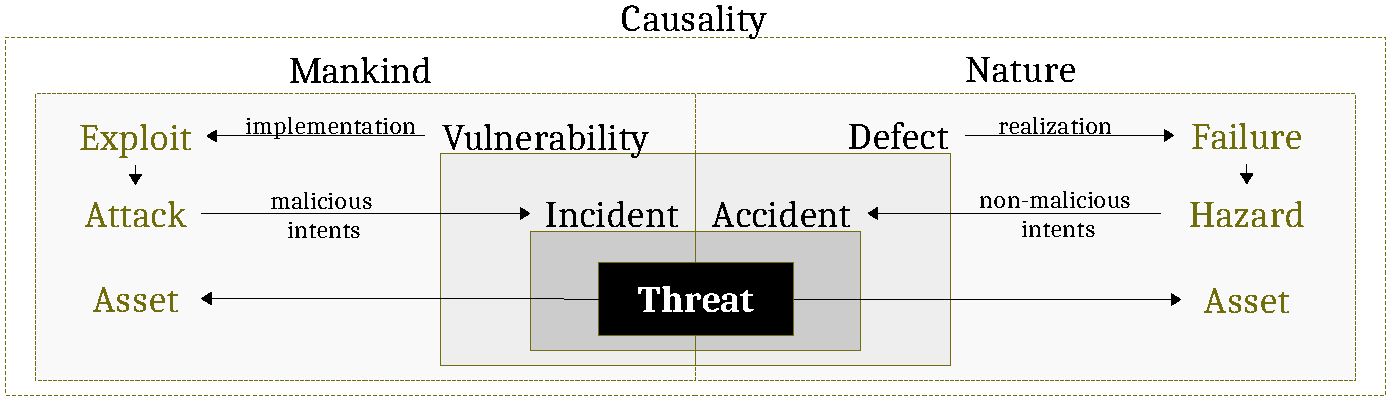
\includegraphics[width=\textwidth]{safety-security.pdf}
	\caption{Overview security and safety keywords}
	\label{fig:safety-security}
\end{figure}

Most of the safety-preserving principles in the field of engineering of
safety-critical cyber-physical systems (such as elevators and aircraft), upon
which safety requirements (e.g. in standards such as the IEC 61508 or 61511\autocite{IEC201761511}) are defined, have
been defined following empirical tests and measurements. While reasoning by
induction based on the empirical observation should be avoided, since it may
easily lead to false beliefs instead of scientific theories, this approach is
often justified by the supposed impossibility of defining a theory that
correctly predicts failures which, in turn, pose hazards to a system. 
To the best of our knowledge, and supported by\autocite{Herley2016unfalsifiability}, the
correlation between predictability of environment and believed unpredictability
of attackers (i.e. a malicious
environment) has not been correlated to a theory on cybersecurity. 
Therefore, inductive research efforts in
predicting malicious effects are accepted (and published) in scientific
conferences (e.g.~\autocite{Rocchetto2014CSRF}). A failure of a wire due to
environment (e.g. due to humidity, dust, heat \&c) is defined from empirical
evidences and processes have been standardized to test qualities of hardware components
%convinced by the induction principle. What is already a
%weak argument in general, 
This process completely breaks down when a malicious environment (i.e. an attacker)
is considered instead of the (supposedly honest and predictable)
natural environment. Therefore, the same approach that is in use for safety,
seems not to be applicable to test security.

Going back to Figure~\ref{fig:safety-security}, a vulnerability does not
necessarily become a threat for the system, unless exploited ``through a
channel that allows the violation of the security policy
[\ldots]''\autocite{cnssi20104009} (e.g. a software or procedure) that takes
advantage of the vulnerability causing an \emph{attack} to the system, which may
result in several correlated incidents and threats.  The process of
exploitation of a defect as a vulnerability is reported in
Figure~\ref{fig:safety-security} such that the difference between exploit and failure,
and attack and accident is to be found just in the maliciousness of the intents
that causes this process (i.e. excluding the intent, the terms are just syntactic transformation from a vulnerability to defect, from
accident to incident). In the following, we conclude the informal definition of
the terms that we used in this section and in Figure~\ref{fig:safety-security}.

\begin{itemize}
	\item \emph{Causality} refers to the causality principle; defined
		in\autocite{Spirkin1983Dialectical} as ``Causality is a genetic
		connection of phenomena through which one thing (the cause)
		under certain conditions gives rise to, causes something else
		(the effect). The essence of causality is the generation and
		determination of one phenomenon by another. In this respect
		causality differs from various other kinds of connection, for
		example, the simple temporal sequence of phenomena, of the
		regularities of accompanying processes''.
	\item An \emph{Exploit}\footnote{We note that the term exploit is only
		used as a verb in\autocite{ISO2009information}} is ``An exploit
		(from the English verb to exploit, meaning to use something to
		one’s own advantage) is a piece of software, a chunk of data,
		or a sequence of commands that takes advantage of a bug or
		vulnerability to cause unintended or unanticipated behavior to
		occur on computer software, hardware, or something electronic
		(usually computerized).''\autocite{wiki-exploit}.
	\item An \emph{Attack}, as defined by the International Standard
		ISO/IEC 27000 is an ``attempt to destroy, expose, alter,
		disable, steal or gain unauthorized access to or make
		unauthorized use of an asset''; where an \emph{Asset} is
		``anything that has value to the organization''. We note that for
		the purpose of this article, we do not want to focus on a specific
		organization or business to define asset but, in general, on any 
		abstract organization (e.g. a company or a society).
		We do not consider ethical hackers as attacking a system. 
		In fact, we consider the term \emph{hack} as
		non-malicious (see Hacker\autocite{Stallman2002hacker}).
	\item A \emph{Threat}, as defined in\autocite{cnssi20104009}, is ``Any
		circumstance or event with the potential to adversely impact
		organizational operations (including mission, functions, image,
		or reputation), organizational assets, individuals, other
		organizations, or the Nation through an information system via
		unauthorized access, destruction, disclosure, modification of
		information, and/or denial of service''.
	\item \emph{Defect}, ``anything that renders the product not reasonably
		safe''\autocite{Robinson2019writing} (i.e. a characteristic of
		an object which hinders its proper usability).
	\item \emph{Failure}, as defined in\autocite{Merriam2020failure} as ``a state of
		inability to perform a normal function''. The term is
		structured and detailed in
		\autocite{cnssi20104009,iet2017glossary} but relying on an
		abstract notion of failure without a specific definition.
	\item \emph{Hazard}, ``a potential source of
		harm''\autocite{iet2017glossary}.
\end{itemize}

\subsection{Glossary -- A Formalization}\label{sec:glossary}
We now define a formalizations of the concepts described in
Section~\ref{sec:problem} and depicted in Figure~\ref{fig:safety-security}. We
base our formalization on first order logic (FOL) with the standard
truth-value semantics. The choice of this logic is required by the 
semantics of the concepts formalized afterwards in this section. 

We consider a first-order language $\follang$ over a
signature $\Sigma_P$ where $P,P',\ldots,P^n$ represent terms, and
$\varphi,\varphi',\ldots,\varphi^n$ represent formulas.
The syntax is defined as follows.
\begin{displaymath}
	\varphi := P~|~\neg\varphi~|~\varphi\wedge\varphi~|~\varphi\vee\varphi~|~\varphi\Rightarrow\varphi'~|~\forall P.~\varphi~|~\exists P.~\varphi
\end{displaymath}
where $\wedge$, $\neg$, $\vee$, and $\Rightarrow$ are connectives representing
conjunction, negation, disjunction, and (material) implication respectively; while
$\forall$ and $\exists$ represent the standard universal and existential
quantifiers (resp.). Finally, the symbol ``$.$'' is just syntactic sugar. 
We consider $\interpretation\subset\Phi\times\{\top,\bot\}$ as the interpretation
function, where $\Phi$ is any collection of sentences in $\follang$ 
and $\top$ and $\bot$ represent the concepts of ``Tautology/True''
and ``Contradiction/False'' respectively.

Following Figure~\ref{fig:safety-security}, we start by formalizing the outermost term: Causality.

\subsubsection{Causality Principle}\label{sec:causality}
We formalize the Causality Principle starting from a K modal
logic\autocite{Garson2018modal} (i.e. without restrictions on the causality
relation between worlds). The standard definition of K modal logic is given in
Definition~\ref{def:modallogic} in terms of an interpretation function (which
we named $\sigma$ with a slight abuse of notation) defined in
Definition~\ref{def:modalinterpretation}. 
\begin{definition}{\bf K Modal Logic --}\label{def:modallogic}
A K-frame is a frame $ \kframe=\langle \possibleworlds,\modalrelation \rangle $
	in the K modal logic where $ \modalrelation $ is the binary relation
	(i.e. a set of ordered pairs) between possible worlds
	$\modalrelation\subseteq\possibleworlds\times\possibleworlds$, where
	$\possibleworlds$ represents the possible worlds, and
	$\possibleworlds\neq\emptyset$. An actual world
	$\actualworld\in\possibleworlds$ is assumed. For any proposition $P$,
	an interpretation function $\interpretation(\world,P)$ returns the
	truth value of $P$; e.g. $\interpretation(\world,P)=\top$ means that
	$P$ holds in $\world$. A model is defined as the tuple
	$\kmodel=\langle\possibleworlds,\modalrelation,\interpretation\rangle$.
\end{definition}

\begin{definition}{\bf Causality as K Modal Interpretation Function --}\label{def:modalinterpretation}
	Causality is (recursively) defined as the modal interpretation function $\interpretation$, as follows. 
	\begin{enumerate}[noitemsep]
		\item[$(\interpretation0)$] if $\interpretation(\world,P)=\top$ then $\world\models P$
		\item[$(\interpretation1)$] $\world\models\neg P$ iff $\world\not\models P$
		\item[$(\interpretation2)$] $\world\models P \wedge Q$ iff $\world\models P$ and $\world\models Q$
		\item[$(\interpretation3)$] $\world\models\Box P$ iff for any world $\world'\in\possibleworlds$ if $\world \modalrelation\world'$ then $\world'\models P$
		\item[$(\interpretation4)$] $\world\models\Diamond P$ iff there exists a set of worlds $\World'\subset\possibleworlds$ such that for any $\world'\in\World'$, if $\world\modalrelation\world'$ then $\world'\models P$
		\item[$(\interpretation5)$] $\models P$ iff $\actualworld\models P$
	\end{enumerate}
	where truth is defined as necessary with $\Box$ and possible with $\Diamond$.
\end{definition}

%\begin{definition}{\bf Causality --}\label{def:causality}
%	The Causality principle is defined over a K Modal Logic (i.e. without
%	restrictions on the causality relation between worlds) as in
%	Definition~\ref{def:modallogic}, with the standard interpretation
%	function defined in~\ref{def:modalinterpretation}
%\end{definition}

The causality principle has been defined in its
generic form. In fact, the accessibility relation $\modalrelation$ is free from
any axiomatic restriction (e.g. it's not reflexive nor anti-reflexive).  
We will focus in Section~\ref{sec:process} (for our tests) on 
the application of our theory to CPS system engineering.
More detailed case studies (i.e. \fix{mr}{a CPS as a smart power-grid}) 
will be defined in Section~\ref{sec:prototest}, where
the accessibility relation defines in details how the system itself evolves, due to causal relation 
(i.e. by restricting the causality principle only to those cause-effect that defines
the system). Therefore, the definition of $\modalrelation$
will be specialized in a more strict way based on the application domains and case study.

We note that we have defined the
Causality principle without considering it a \emph{threat source} since 
we lack the concept of intent and maliciousness. Similarly, in the 
next sections we won't discriminate between Nature and Mankind until we introduce 
the concepts of maliciousness in Section~\ref{sec:theory} 
and then formally define a threat agent
in the same section.

\subsubsection{Agents: Mankind and Nature}\label{sec:mankind-nature}
\begin{table}[t]
\centering
\setlength{\tabcolsep}{3.5pt}
\renewcommand{\arraystretch}{1}
\scriptsize
\caption{RCC3, RCC5, and RCC8 relations between Regions $X$, $Y$ and $Z$ ~\label{tab:rcc358}~\label{tab:rcc}}
\begin{tabular}{ccclll} 
\rota{\textbf{RCC3}}&\rota{\textbf{RCC5}}&\rota{\textbf{RCC8}}&\textbf{Name} & \textbf{Notation} & \textbf{Definition} \\
\hline
&&&Connects with 			& $\mathit{C}(\mathit{X},\mathit{Y})$ 		& $\mathit{X}\subseteq \mathit{Y}$ \\
&&&Disconnected from		& $\neg \mathit{C}(\mathit{X},\mathit{Y})$		& $\mathit{X}\not\subseteq \mathit{Y}$\\
&&&Part of				& $\mathit{P}(\mathit{X},\mathit{Y})$		& $\forall \mathit{Z} ~\mathit{C}(\mathit{Z},\mathit{X}) \rightarrow \mathit{C}(\mathit{Z},\mathit{Y})$\\
&&&Overlaps			& $\mathit{O}(\mathit{X},\mathit{Y})$		& $\exists \mathit{Z} ~\mathit{P}(\mathit{Z},\mathit{X})\wedge \mathit{P}(\mathit{Z},\mathit{Y})$\\
\Tdot&&&  \textbf{Overlaps Not Equal} 	& $\mathit{ONE}(\mathit{X},\mathit{Y})$		& $\mathit{O}(\mathit{X},\mathit{Y}) \land \neg \mathit{EQ}(\mathit{X},\mathit{Y})$ \\
\Tdot&\Tdot&\Tdot& \textbf{Equal to} 		& $\mathit{EQ}(\mathit{X},\mathit{Y})$  		& $\mathit{P}(\mathit{X},\mathit{Y}) \wedge \mathit{P}(\mathit{Y},\mathit{X})$\\
\Tdot&\Tdot&\Tdot& \textbf{DiscRete from} 		& $\mathit{DR}(\mathit{X},\mathit{Y})$		& $\neg \mathit{O}(\mathit{X},\mathit{Y})$\\
&\Tdot&\Tdot&\textbf{Partial-Overlap}	& $\mathit{PO}(\mathit{X},\mathit{Y})$ 		& $\mathit{O}(\mathit{X},\mathit{Y})\wedge \neg \mathit{P}(\mathit{X},\mathit{Y}) \wedge \neg \mathit{P}(\mathit{Y},\mathit{X})$\\ 
&\Tdot&&\textbf{Proper-Part-of} 	& $\mathit{PP}(\mathit{X},\mathit{Y})$ 		& $\mathit{P}(\mathit{X},\mathit{Y})\wedge \neg \mathit{P}(\mathit{Y},\mathit{X})$\\ 
	&\Tdot&&\textbf{Proper-Part-of-\textit{\textbf{i}}nverse} & $\mathit{PPi}(\mathit{X},\mathit{Y})$ 		& $\mathit{P}(\mathit{Y},\mathit{X}) \wedge \neg \mathit{P}(\mathit{X},\mathit{Y})$\\
&&\Tdot&\textbf{Externally Connected} 	& $\mathit{EC}(\mathit{X},\mathit{Y})$ 		& $\mathit{C}(\mathit{X},\mathit{Y}) \wedge \neg\mathit{O}(\mathit{X},\mathit{Y})$\\ 
&&\Tdot&\textbf{Tangential PP} 	& $\mathit{TPP}(\mathit{X},\mathit{Y})$ 		& $\mathit{PP}(\mathit{X},\mathit{Y})\wedge\exists\mathit{Z}~[\mathit{EC}(\mathit{Z},\mathit{X}),\mathit{EC}(\mathit{Z},\mathit{Y})]$\\ 
&&\Tdot&\textbf{Tangential PPi} 	& $\mathit{TPPi}(\mathit{X},\mathit{Y})$ 		& $\mathit{TPP}(\mathit{Y},\mathit{X})$\\ 
&&\Tdot&\textbf{Non-Tangential PP} 	& $\mathit{NTPP}(\mathit{X},\mathit{Y})$ 		& $\mathit{PP}(\mathit{X},\mathit{Y})\wedge\neg\exists\mathit{Z}~[\mathit{EC}(\mathit{Z},\mathit{X}),\mathit{EC}(\mathit{Z},\mathit{Y})]$\\ 
&&\Tdot&\textbf{Non-Tangential PPi} 	& $\mathit{NTPPi}(\mathit{X},\mathit{Y})$ 		& $\mathit{NTPP}(\mathit{Y},\mathit{X})$\\ 
\end{tabular}
\end{table}

Mankind and Nature are defined in Section~\ref{sec:problem} as two abstract
agents, both as collections (i.e. an abstract type that does not imply a
specific implementation) of their sub-agents (i.e. humans for Mankind and
plants, animals, \&c.  for Nature). Similarly to\autocite{Santaca2016abf}, 
we define Mankind and Nature, and any
other agent in the reminder of this article, as a meronomy (an hierarchy of
Part-Whole relations) based on a standard definition of mereology, i.e. based
on the definition of Parthood relation between \emph{Parts}.  
However, shall 
consider different types of Part; so, we extend the mereology to a
mereo-topology\autocite{Smith1996mereotopology,Varzi1994mereotopology,Rachavelpula2017mereotopology},
to increase the number of different types considered and to generalize the relations between Parts (as
in Table~\ref{tab:rcc358}).
For the sake of readability, we use the term \emph{Region} both to refer to a
mereological Part and to a topological Region.
The choice of mereotopology is also correlated to the objective of defining a formal
ontology, which we use to define the (formal) semantics of the terms (Parts) in
Section~\ref{sec:problem}, and of the concepts of safety and security
(whole). We aim at creating a meronomy instead of the taxonomies such as the one provided
in\autocite{NIST2020NVD,MITRE2020CVE} or instead of the poorly justified 
CVSS\autocite{Mell2007CVSS} scoring system.  

A mereotopology, as defined e.g. in\autocite{Rachavelpula2017mereotopology},
is an ordered mathematical structure where the basic relation between Regions is the
reflexive and symmetric\fixnote{mr}{I guess it must be monotonic as defined in\autocite{Rachavelpula2017mereotopology} but I don't find it consistently in other papers.} 
\emph{Parthood} relation $\subseteq$. 
\begin{definition}{\bf Parthood --}\label{def:parthood}
Given any pair of mereotopological Regions $X$ and $Y$,
	\begin{enumerate}[noitemsep]
		\item Reflexivity: $\forall X.~ (X\subseteq X)$
		\item Symmetry: $\forall X, Y.~ (X\subseteq Y \Rightarrow Y\subseteq X)$
	\end{enumerate}
\end{definition}

As later defined in Definition~\ref{def:agent}, 
the Parthood relation orders a universe of agents $\agentuniverse$ by defining
the so called \emph{Connects with} (see in Table~\ref{tab:rcc358}) relation 
between Regions. We want this universe $\agentuniverse$ to be 
expressible in FOL. In this way, we
can reason both on the constituent of security (i.e. its terms and agents
defining a system where security needs to be considered), and on 
the evolution of those constituent w.r.t. cause-effects relations according
to the modal structure of causality we defined in Section~\ref{sec:causality}.
This will allow us (in Section~\ref{sec:process} and Section~\ref{sec:prototest})
a better\fixnote{mr}{Can we prove this by construction?} 
positioning w.r.t. risk assessment technologies
(which most often reason on the constituent of a system design), and
protocol verification tools (which requires some formalization of a cause-effect relation, e.g.
in Linear Temporal Logic).

As we argued in Section~\ref{sec:problem}, we must correlate the definition of
agent (i.e. Mankind and Nature) in Definition~\ref{def:mankind-nature} to the
mathematical structure of the logic that defines them.  We express Mankind and
Nature as formulas over the theory of mereology and then in terms of
mereotopological Regions, extending the interpretation function
$\interpretation$, to include a formal theory of mereotopology.  We use the
Region Connection Calculus (RCC), as defined
in~\cite{bennettLogics,improvingRCC}, to provide an axiomatization of the
spatial concepts and relations in first-order logic to correlate the algebraic
structure to mereology. In its broader definition, the RCC theory is composed
by eight axioms, and is known as RCC8. In the text, for brevity, 
we will often focus only on RCC5 (without
loss of generality) by not considering tangential connections between spatial
Regions. We discuss the choice of RCC5 in more detail in
Appendix~\ref{app:rcc}. In Table~\ref{tab:rcc}, we
summarize the axioms of the Region Connection Calculus (see, e.g., \autocite{Grutter2008rcc}).

\begin{definition}{\bf RCC axiomatization --}
	For any $X,Y$ pair of Regions in a mereotopology:
	\begin{itemize}[noitemsep]
	\item[$(\interpretation6)$] $\interpretation(X\subseteq Y)$ iff [$\interpretation(X\subseteq X)=\top$, and $\interpretation(X\subseteq Y)=\bot$ or $\interpretation(Y\subseteq X)=\top$]\fixnote{mr}{would it be better/clearer or just correct to write $\sigma(X\subseteq Y)$ iff $\sigma(X\subseteq X\wedge [X\subseteq Y \vee Y\subseteq X])=\top$}
	\item[$(\interpretation7)$] $\world\models\connects{X}{Y}$ iff $\world\models X\subseteq Y$ 
	\item[$(\interpretation8)$] $\world\models\disconnected{X}{Y}$ iff  $\world\not\models X\subseteq Y$
	\item[$(\interpretation9)$] $\world\models\partof{X}{Y}$ iff $\world\models\forall Z.~\connects{Z}{X}\Rightarrow\connects{Z}{Y}$
	\item[$(\interpretation10)$] $\world\models\overlaps{X}{Y}$ iff $\world\models\exists Z.~\partof{Z}{X}\wedge\partof{Z}{Y}$
	\item[$(\interpretation11)$] $\world\models\eq{X}{Y}$ iff $\world\models\partof{X}{Y}\wedge\partof{Y}{X}$
	\item[$(\interpretation12)$] $\world\models\dr{X}{Y}$ iff $\world\models\neg\overlaps{X}{Y}$
	\item[$(\interpretation13)$] $\world\models\po{X}{Y}$ iff $\world\models\overlaps{X}{Y}\wedge\neg\partof{X}{Y}\wedge\neg\partof{Y}{X}$
	\item[$(\interpretation14)$] $\world\models\pp{X}{Y}$ iff $\world\models\partof{X}{Y}\wedge\neg\partof{Y}{X}$
	\item[$(\interpretation15)$] $\world\models\ppi{X}{Y}$ iff $\world\models\partof{Y}{X}\wedge\neg\partof{X}{Y}$
\end{itemize}
where $Z$ is a mereotopological Region.
\end{definition}

\begin{definition}{\bf Agent: Mankind or Nature --}\label{def:agent}
	An agent $\agent\in\agentuniverse$ is a tuple
	$\langle\rcc(\region',\region''),\ldots,\rcc(\region^{n-1},\region^n)\rangle$
	of RCC relations $\rcc$ over mereotopological Regions
	${\region',\ldots,\region^n}\subseteq\Region$. 
\end{definition}

Currently, we do not distinguish between Mankind and Nature (since we still
lack of the definition of ``malicious intent'', which is defined in
Section~\ref{sec:theory}) and we have defined them as two generic
agents.

As depicted in Figure~\ref{fig:safety-security}, Causality, Mankind, and Nature
have a dashed border representing their correlation in terms of cause-effect
and then in terms of formal structure which defines them: Modal Logic.
Vulnerability, Defect, Incident, Accident, and Threat, similarly, 
are correlated (depicted as a solid border) in terms of underlying 
formal structure: Mereotopology.

\subsubsection{Regions: Vulnerability and Defect (and Weakness)}\label{sec:vulnerabilitydefect}
As defined in Section~\ref{sec:problem}, a Vulnerability or a Defect is a
\emph{Weakness}.  As an example, a categorization of weaknesses is given
in\autocite{MITRE2020CWEresearch} with 808 weaknesses categorized as ``Research
Concepts'', distributed as follows:
\begin{itemize}[noitemsep]
	\item Incorrect Calculation - ($682$)
	\item Incorrect Access of Indexable Resource (``Range Error'') - ($118$)
	\item Use of Insufficiently Random Values - ($330$)
	\item Improper Interaction Between Multiple Correctly-Behaving Entities - ($435$)
	\item Improper Control of a Resource Through its Lifetime - ($664$)
	\item Insufficient Control Flow Management - ($691$)
	\item Protection Mechanism Failure - ($693$)
	\item Incorrect Comparison - ($697$)
	\item Improper Check or Handling of Exceptional Conditions - ($703$)
	\item Improper Enforcement of Message or Data Structure - ($707$)
	\item Improper Adherence to Coding Standards - ($710$)
\end{itemize}

The definition given by the MITRE in\autocite{MITRE2020CWEweakness} of
weakness is: ``Software weaknesses are errors that can lead to software
vulnerabilities. A software vulnerability, such as those enumerated on the
Common Vulnerabilities and Exposures (CVE) List, is a mistake in software that
can be directly used by a hacker to gain access to a system or network''.
The definition is circular if we interpret the word ``error'' and
``mistake'' with the same semantics: a weakness is an error that leads to a
vulnerability and a vulnerability is a mistake which, in turn, is a weakness.
The only difference (between weakness and vulnerability) seems to be
that one can consider weakness as a ground term and state that a
vulnerability is caused by a weakness, i.e. 
$\World,\Weakness\models\Diamond\Vulnerability\wedge\Weakness$ where
$\Weakness,\Vulnerability$ are Regions of Weaknesses and Vulnerabilities (resp.);
accepting the hierarchy in the CWE\autocite{CWE} as ground truth. 
Similarly, we consider the CVE\autocite{CVE} (a database of Vulnerability) 
or the CVE reported in the NVD as a ground truth. 

\begin{definition}{\bf Region: Weakness and Vulnerability --}\label{def:weakness}
	A Region $\region\subseteq\agent$ of an agent
	$\agent\in\agentuniverse$, is defined as Weakness $\Weakness$ (i.e.
	representing a weakness introduced by the agent into any phase of
	production, e.g.  of the secure process development life-cycle, of any
	system or subsystem) iff there exists $\world\in\possibleworlds$ such
	that $\world,\Weakness\models\Diamond\exists\Weakness',\Vulnerability'.~
	\rcc(\Weakness',\Vulnerability')\wedge\neg\dr{\Weakness'}{\Vulnerability'}$, 
	where $\Weakness'\subseteq\Weakness$, and
	$\Vulnerability'\subseteq\Vulnerability$ is a Region of an agent $\agent'\in\agentuniverse$.
\end{definition}

\begin{example}{CWE-116: Improper Encoding or Escaping of Output\autocite{CWE-116} --}
	\begin{itemize} 
		\item Description: The software prepares a structured message
		for communication with another component, but encoding or
		escaping of the data is either missing or done incorrectly. As
		a result, the intended structure of the message is not
		preserved. 
		\item Example: This code displays an email
		address that was submitted as part of a form. Example language JSP.
		\begin{verbatim} 
		<% String email = request.getParameter("email"); %> 
		...
		Email Address: <%= email %>
		\end{verbatim}
		The value read from the form parameter is
		reflected back to the client browser without
		having been encoded prior to output, allowing
		various XSS attacks (CWE-79).
		\item Observed Examples
			\begin{itemize}
			\item CVE-2008-4636\autocite{CVE-2008-4636}: OS command injection in backup
				software using shell metacharacters in a
				filename; correct behavior would
				require that this filename could not be
				changed.
			\item CVE-2008-0769\autocite{CVE-2008-0769}: Web application does not set the
				charset when sending a page to a browser,
				allowing for XSS exploitation when a
				browser chooses an unexpected encoding.
			\item CVE-2008-0005\autocite{CVE-2008-0005}: Program does not set the charset
				when sending a page to a browser, allowing for
				XSS exploitation when a browser chooses
				an unexpected encoding.
			\item CVE-2008-5573\autocite{CVE-2008-5573}: SQL injection via password
				parameter; a strong password might contain \&
			\item CVE-2008-3773\autocite{CVE-2008-3773}: Cross-site scripting in chat
				application via a message subject, which
				normally might contain \& and other
				XSS-related characters.
			\item CVE-2008-0757\autocite{CVE-2008-0757}: Cross-site scripting in chat
				application via a message, which normally might
				be allowed to contain arbitrary
				content.
			\end{itemize}
\end{itemize}

\begin{figure}[t]
	\centering
	\begin{subfigure}[b]{.5\textwidth}
		\centering
		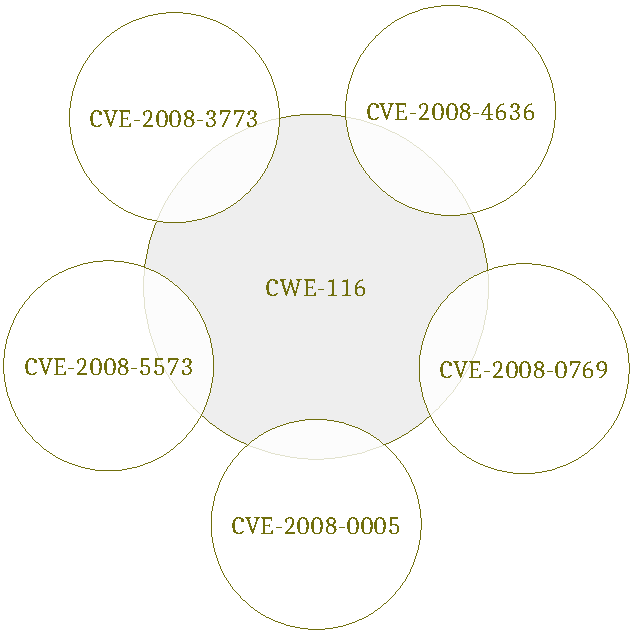
\includegraphics[width=.7\textwidth]{rcc5_CWE-116.pdf}
		\caption{Representation with RCC3}
		\label{fig:rcc5_CWE-116}
	\end{subfigure}\begin{subfigure}[b]{.5\textwidth}
		\centering
		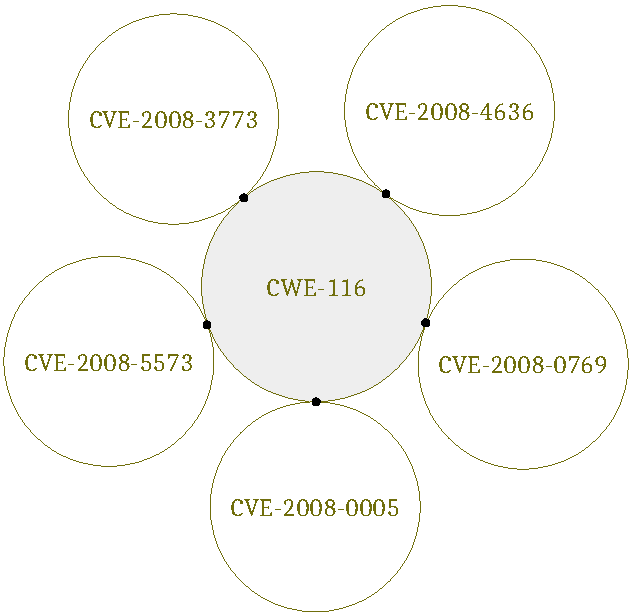
\includegraphics[width=.7\textwidth]{rcc8_CWE-116.pdf}
		\caption{Representation with RCC8}
		\label{fig:rcc8_CWE-116}
	\end{subfigure}
	\begin{subfigure}[b]{\textwidth}
		\centering
		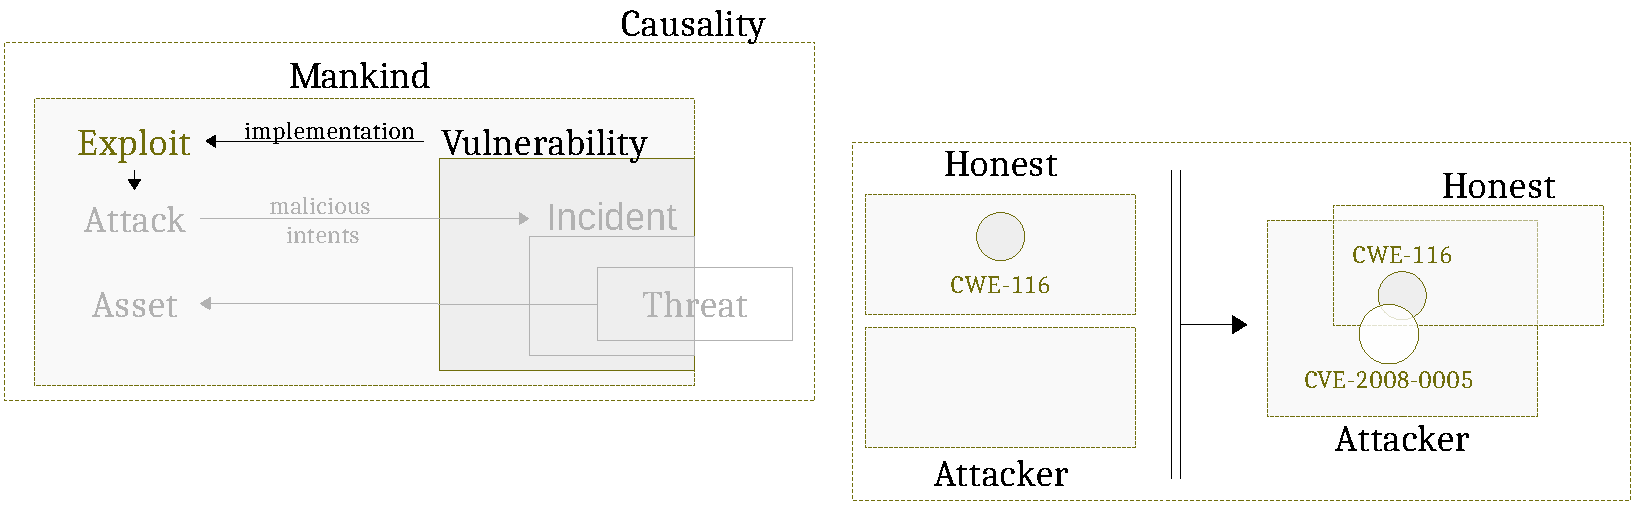
\includegraphics[width=\textwidth]{KML_CWE-116.pdf}
		\caption{Representation in K-Modal Logic}
		\label{fig:KML_CWE-116}
	\end{subfigure}
	\caption{Relations between CWE-116 and correlated CVEs}
\end{figure}
Definition~\ref{def:weakness} states that CWE-116 is a weakness iff there exists a world in
K Modal Logic, representing the system in which this weakness exists, 
such that the natural evolution of this system (i.e. formalized by the causality principle) 
make it possible to reach another state of the system (i.e. another, accessible world)
where there exist a vulnerability that can be implemented from CWE-116 (and this relation 
is not DR). The CWE website proposes the connection between CWE-116 and, for example, 
CVE-2008-5573; a vulnerability of the login sub-system 
of the Poll Pro v2.0\autocite{pollpro} system.
The formal relation between the two is given as a link (i.e. URI) between the CWE and
the CVE, the description of the relation is not defined but it is supposed to be
inferred from the descriptions of the CWE-CVE. 
We can formally represent this link as the ONE connection in RCC3, depicted in 
Figure~\ref{fig:rcc5_CWE-116}, or EC connection in RCC8 (Figure~\ref{fig:rcc8_CWE-116}).

\fixnote{mr}{shouldn't we consider the agent who introduces the weakness as dishonest? don't we say this in part 1?}
\end{example}

It is interesting to note that the CWE-CVE relation expresses the correlation
between weaknesses and vulnerabilities in the most simple form, such that we
can formalize all the relation as ONE in RCC3 or EC in RCC8.  To express a more
complex relation between the two we shall analyze the definition of CWE-116.
This is related to the Weakness-Vulnerability-Incident process (i.e. to the
details on the implementation/realization in Figure~\ref{fig:safety-security})
that we analyze in the next section, Section~\ref{sec:incidentaccident}.

\begin{definition}{\bf Region: Vulnerability and Defect --}\label{def:vulnerability-defect}
A region $\region\subseteq\agent$ of an agent $\agent\in\agentuniverse$ is
	called \emph{Vulnerability} if the agent $\agent$ is referred to as Mankind, 
	\emph{Defect} if the agent is referred to as Nature.
\end{definition}

\subsubsection{Process: Incidents and Accidents}\label{sec:incidentaccident}
In our informal definition depicted in Figure~\ref{fig:safety-security}, an
Incident is generated through a process caused by a Vulnerability (which,
in turn, is caused by a Weakness). Symmetrically, Nature has a process from Defect
to Accidents. We start by analyzing the process generated by Mankind, which is
divided into the following phases (as shown in Figure~\ref{fig:cwe-nvd-capec}):
\begin{enumerate}
	\item An agent (Mankind or Nature) defines a system, e.g. by following an engineering process for creating a new system, or for redesigning or improving an existing system (e.g. a component or a collection of components) 
	\item The dogmatic definition of a system contains a Weakness (i.e. the agent, Mankind or Nature, introduces an unintended behavior), for example as an un-intended behavior or as an architectural fallacy. The Weakness can be applied to the abstract definition of the system.
	\item The Weakness can be defined as a malicious process for a system, called Vulnerability (or Defect for Nature)
	\item The process expressed by the Vulnerability can be made operational for a specific implementation of the system (i.e. implemented by Mankind or realized by Nature) 
\end{enumerate}
Those additional details are depicted in Figure~\ref{fig:safety-security_2}, an update
of Figure~\ref{fig:safety-security}.

\begin{figure}[t]
	\centering
	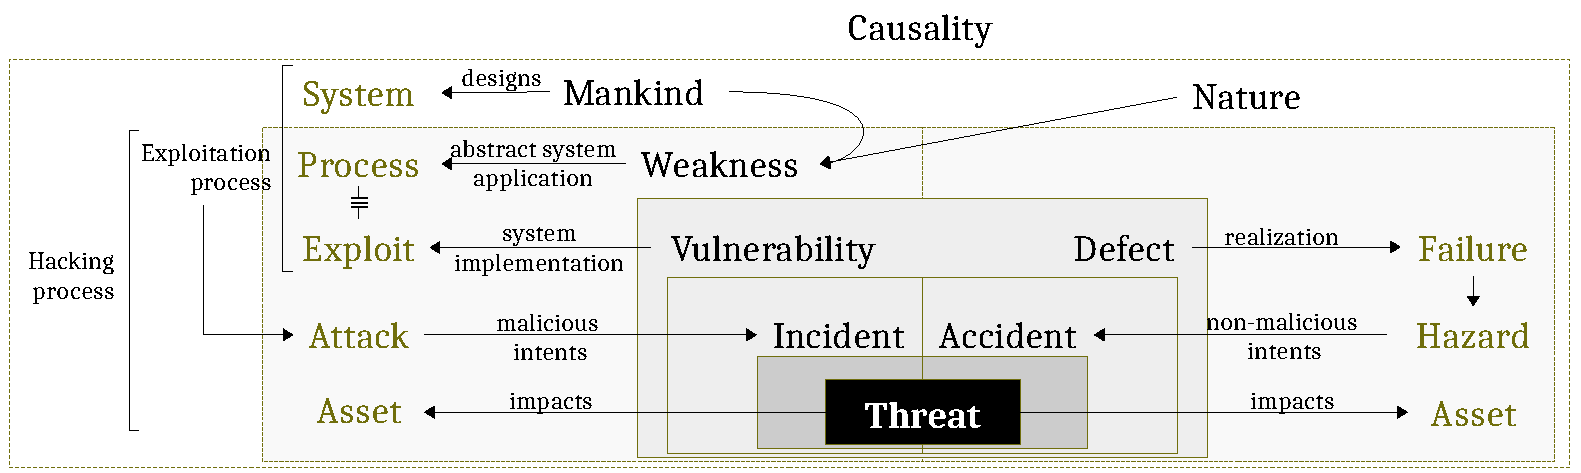
\includegraphics[width=\textwidth]{safety-security_2.pdf}
	\caption{Updated overview security and safety keywords, where Process
	has to be intended as ``Abstract Exploitation Process''}
	\label{fig:safety-security_2}
\end{figure}

\begin{definition}{\bf Exploitation Process --} An \emph{Exploit} is an \emph{implementation} of
a Vulnerability, where a Vulnerability describes how to transform a
Weakness into an abstract malicious process, which can be applied\footnote{Meaning that the
malicious process, i.e.  any structured procedure such as a protocol, can be
somehow made operational, e.g. implemented} to one or many systems. So, the act
of an agent (Mankind) of ``exploiting a Vulnerability'' is the process of
making the Vulnerability operational, by implementing the Vulnerability w.r.t.
a specific target system.  Whenever the agent is Nature, the implementation is
more broadly considered a realization\footnote{``The state of being
realized''\autocite{Merriam2020realization}}. 
\end{definition}

The Common Attack Pattern Enumeration and
Classification\autocite{MITRE2020CAPEC} (CAPEC) online service provides a
``community resource'' which aims at ``identifying and understanding attacks''.
The MITRE writes on the CAPEC homepage that ``Understanding how the adversary
operates is essential to effective cyber security. CAPEC helps by providing a
comprehensive dictionary of known patterns of attack employed by adversaries to
exploit known weaknesses in cyber-enabled capabilities. It can be used by
analysts, developers, testers, and educators to advance community understanding
and enhance defenses.''. We can extrapolate two major concepts: 
\begin{itemize}
	\item While understanding the exploitation process is the aim of the
		CWE and CVE initiatives, understanding the hacking process is
		the aim of the CAPEC initiative.
	\item CAPEC provides a \emph{dictionary} of \emph{known} attack patterns.
		As stated in details in Section~\ref{sec:problem}, this dictionary contains
		empirical evidences and should not be used to induce a cybersecurity 
		theory; but it can be used to validate a theory.
\end{itemize}

\begin{example}
The CWE-116 doesn't just relate the Weakness to a number of Vulnerability in
	the CVE but also relates the Weakness to a number ($4$ for the CWE-116)
	of abstract attack path in the CAPEC:
	\begin{itemize}
		\item CAPEC-104\autocite{CAPEC-104} Cross Zone Scripting
		\item CAPEC-73\autocite{CAPEC-73} User-Controlled Filename
		\item CAPEC-81\autocite{CAPEC-81} Web Logs Tampering
		\item CAPEC-85\autocite{CAPEC-85} AJAX Fingerprinting
	\end{itemize}

	Each CAPEC entry has a reference to one or many CWE, including CWE-116.
\end{example}

After the exploitation process, as depicted in Figure~\ref{fig:cwe-nvd-capec},
another process starts and transforms a Vulnerability in an Incident by
Attacking the system with a malicious Hack, as follows.
\begin{enumerate}
\setcounter{enumi}{4}
	\item An agent (Mankind\footnote{For the sake of readability we focus
		only on Mankind as an agent}) the exploitation process can be
		used to hack a system. We use the term hack (as hacking) to
		stress that nothing prevents this process from being honest,
		however, for the sake of simplicity, we focus on Attacks which
		are malicious by definition.
	\item An Attack is applied to a system with malicious intent by an
		agent
	\item The application of the attack results in an Incident which
		impacts, i.e. poses a Threat to, an Asset
\end{enumerate}

\begin{definition}{\bf Hacking Process}\label{def:hackingprocess}
An \emph{Attack} is the act of making operational an \emph{Exploitation Process} 
	causing an Incident. \fix{mr}{Threat? Asset?}
\end{definition}

\begin{example}	CAPEC-81\autocite{CAPEC-81} Web Logs Tampering --
	\begin{itemize}
		\item Description: An attacker is able to cause a victim to
			load content into their web-browser that bypasses
			security zone controls and gain access to increased
			privileges to execute scripting code or other web
			objects such as unsigned ActiveX controls or applets.
			This is a privilege elevation attack targeted at
			zone-based web-browser security. In a zone-based model,
			pages belong to one of a set of zones corresponding to
			the level of privilege assigned to that page. Pages in
			an untrusted zone would have a lesser level of access
			to the system and/or be restricted in the types of
			executable content it was allowed to invoke. In a
			cross-zone scripting attack, a page that should be
			assigned to a less privileged zone is granted the
			privileges of a more trusted zone. This can be
			accomplished by exploiting bugs in the browser,
			exploiting incorrect configuration in the zone
			controls, through a cross-site scripting attack that
			causes the attackers' content to be treated as coming
			from a more trusted page, or by leveraging some piece
			of system functionality that is accessible from both
			the trusted and less trusted zone. This attack differs
			from "Restful Privilege Escalation" in that the latter
			correlates to the inadequate securing of RESTful access
			methods (such as HTTP DELETE) on the server, while
			cross-zone scripting attacks the concept of security
			zones as implemented by a browser. 
		\item Execution Flow: 
			\begin{enumerate}
				\item Explore: Find systems susceptible to the
					attack: Find systems that contain
					functionality that is accessed from
					both the internet zone and the local
					zone. There needs to be a way to supply
					input to that functionality from the
					internet zone and that original input
					needs to be used later on a page from a
					local zone. 
				\item Experiment: Find the insertion point for
					the payload: The attacker first needs
					to find some system functionality or
					possibly another weakness in the system
					(e.g. susceptibility to cross site
					scripting) that would provide the
					attacker with a mechanism to deliver
					the payload (i.e. the code to be
					executed) to the user. The location
					from which this code is executed in the
					user's browser needs to be within the
					local machine zone.
				\item Exploit: Craft and inject the payload:
					Develop the payload to be executed in
					the higher privileged zone in the
					user's browser. Inject the payload and
					attempt to lure the victim (if
					possible) into executing the
					functionality which unleashes the
					payload.
			\end{enumerate}
		\item Prerequisite: The target must be using a zone-aware browser. 
		\item Consequences: 
			\begin{itemize}
				\item Integrity: Modify Data
				\item Confidentiality: Read Data
				\item Confidentiality, Access Control, Authorization: Gain Privileges
				\item Confidentiality, Integrity, Availability: Execute Unauthorized Commands
			\end{itemize}
	\end{itemize}

\end{example}

\begin{figure}[t]
	\centering
	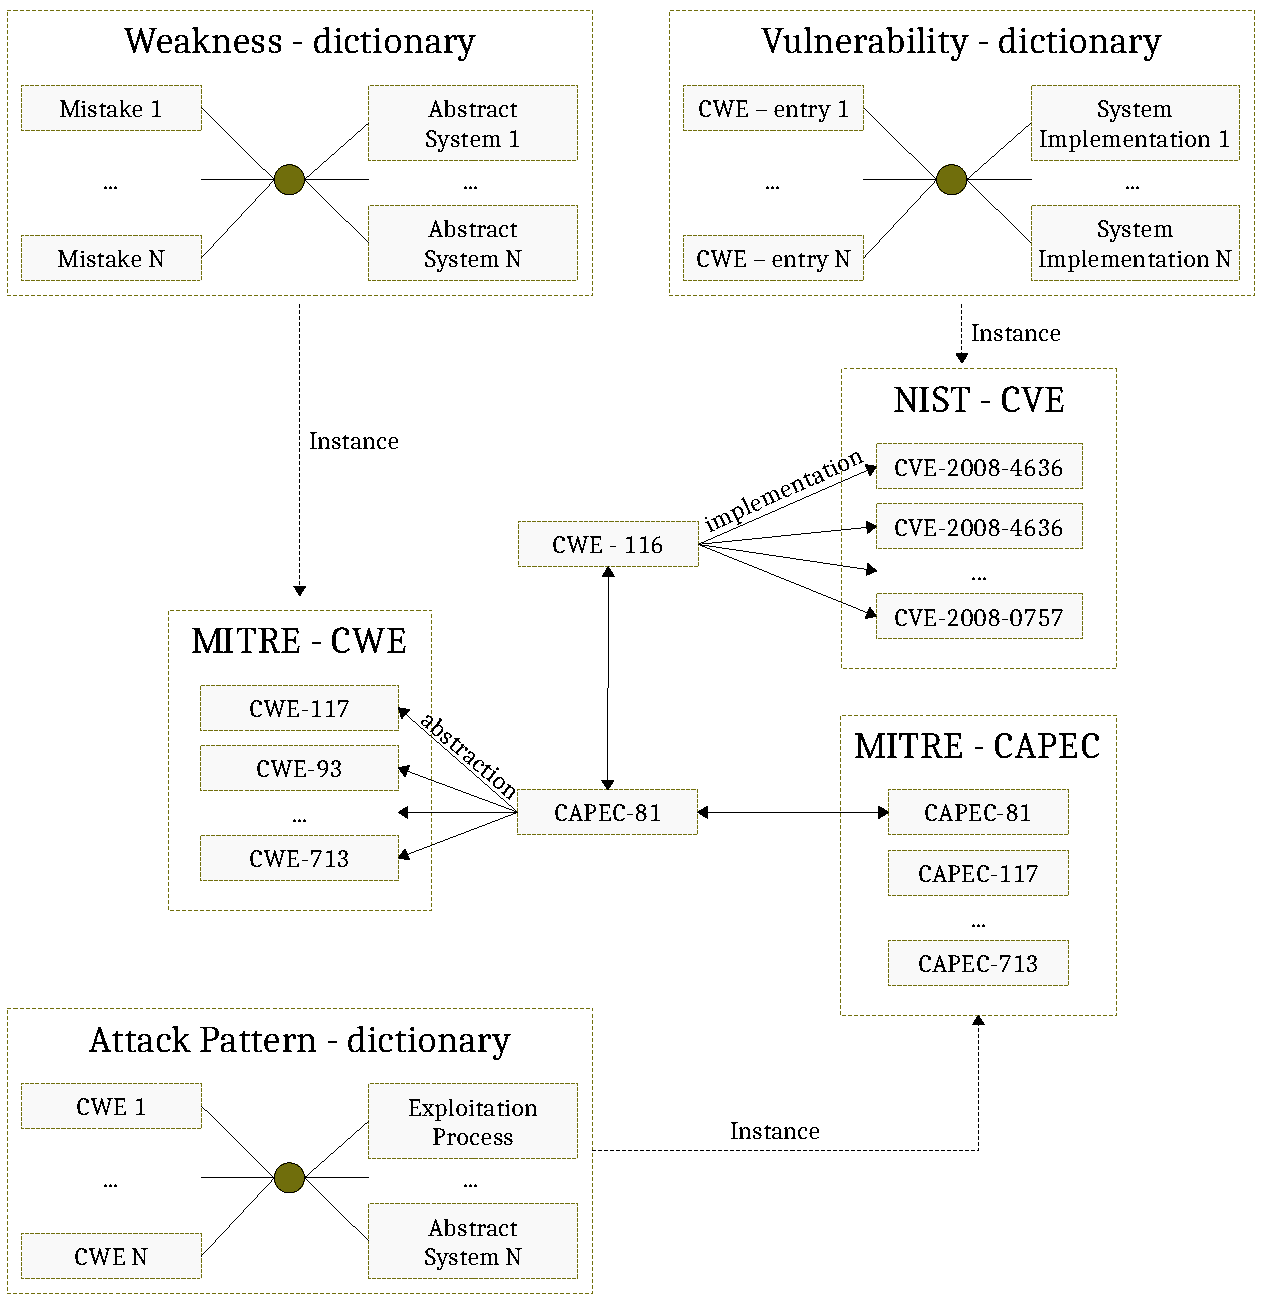
\includegraphics[width=\textwidth]{cwe-nvd-capec.pdf}
	\caption{Cybersecurity online dictionaries and connections}
	\label{fig:cwe-nvd-capec}
\end{figure}

The formalization of the Exploitation and Hacking processes is the
formalization of two foundational cybersecurity concepts which lay the basis
for the definition (and formalization) of the cybersecurity theory in the next
Section (Section~\ref{sec:theory}). However, the formal definition of those
processes shall (i) correlate the formal definition of agents (i.e. the
Definition~\ref{def:agent}) with the Causality principle (i.e. the
formalization of the Kripke structure in Definition~\ref{def:causality}), and,
most importantly, (ii) formally define a system as a structure of agents. For
the sake of clarity, we then postpone the formalization of the two processes to
the next Section.













We describe processes, in our current formalization, in terms of the K-Modal
Structure as in Definition~\ref{def:modalinterpretation} (i.e. in terms of
causality principle). 

\begin{definition}{\bf Vulnerability-Incident Process --}\label{def:vulnerability-incident}
	Given two 
\end{definition}

The whole-part relation \fix{mr}{(i.e.  HAS-A\footnote{HAS-A is just an hint for the
mechanization of this theory.  We'll come back to this in
Section~\ref{sec:implementation}})} is given, in the following, over the K Modal
logic described beforehand. To do so, we first need to formally define the
concept of \emph{agent} in its abstract form. We build it following the same
structure of\autocite{Santaca2016abf} but over the terms used in
Section~\ref{sec:problem}, i.e. knowledge, and belief as epistemic concepts. We'll then 
introduce the concept of \emph{intent} to define a \emph{threat agent}.

\begin{figure}[t]
	\centering
	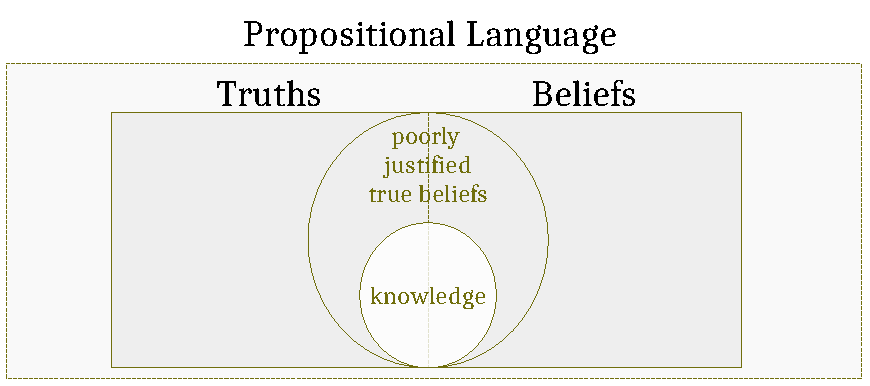
\includegraphics[width=.8\textwidth]{knowledge-belief.pdf}
	\caption{Informal representation of Knowledge and Belief}
	\label{fig:knowledge-belief}
\end{figure}


\subsubsection{Region: Threat and Asset}\label{sec:threatasset}
The difference between Knowledge and Belief is depicted in
Figure~\ref{fig:knowledge-belief} (see \autocite{wiki-knowledgebelief}).  However,
according to\autocite{Gettier2012knowledge},
Knowledge\footnote{``\emph{Theaetetus}: [\ldots] He said that knowledge was
true opinion accompanied by reason, but that unreasoning true opinion was
outside of the sphere of knowledge; and matters of which there is not a
rational explanation are unknowable -- yes, that is what he called them -- and
those of which there is are knowable. [\ldots] \emph{Socrates}: [\ldots] the
primary elements of which we and all else are composed admit of no rational
explanation; for each alone by itself can only be named, and no qualification
can be added, neither that it is nor that it is not, for that would at once be
adding to it existence or non-existence, whereas we must add nothing to it, if
we are to speak of that itself alone.  [\ldots]'' Plato -- Theaetetus 201
\autocite{Plato1914Plato}} as an epistemological concept is difficult (and
sometimes believed impossible\autocite{citation}) to formally define. In this
work, we are not interested in 
how knowledge can be precisely formalized from an epistemic standpoint. 
We assume that a semantic of a correct definition of epistemic knowledge exists,
for example the one given in\autocite{Hintikka1962knwoledge} by Hintikka, and we then define 
knowledge in terms of the Kripke structure defined in Definition~\ref{def:causality}.

\begin{definition}{\bf Knowledge --}\label{def:knowledge}
Given an abstract collection of Agents $Ag$, and the modal operator
	$\knows{a}{}$ (where $a\in Ag$), Knowledge is defined as a collection
	of predicates known by an agent $\knowledge{a}=\bigcup_\Phi \knows{a}{\varphi}$ 
	(where $\Phi$ is the collection of all the propositions known by $a$).
	Given a proposition $P$, we extend the semantics of the Causality structure with:
	\begin{enumerate}[noitemsep]
		\item[$(\interpretation6)$] $\world\models\knows{a}{P}$ iff
			$\world'\models P$ for all $\world'$ such that
			$\world\modalrelation\world'$.
	\end{enumerate}
\end{definition}

\begin{definition}{\bf Belief --}\label{def:belief}
	\fix{mr}{we should help the reader in understanding the upgrades of the logic. We used propositional with modal operators with a K Kripke semantics and we are now introducing Belief as in Doxastic logic? and we have epistemological operators as knowledge}
	Given an abstract collection of Agents $Ag$, and the modal operator
	$\believe{a}{}$ (where $a\in Ag$), Belief is defined as a collection
	of predicates believed by an agent $\belief{a}=\bigcup_\Phi \believe{a}{\varphi}$
	(where $\Phi$ is the collection of all the propositions believed by $a$).
	Given a proposition $P$, we extend the semantics of the Causality structure with:
	\begin{enumerate}[noitemsep]
		\item[$(\interpretation7)$] $\world\models\believe{a}{P}$ iff
			$\world\models\neg\knows{a}{\neg P}$ (i.e. the agent $a$ considers $P$ possible) 
			and $\world'\models P$ for all
			$\world'$ such that $\world\modalrelation\world'$.
	\end{enumerate}
\end{definition}

\begin{definition}{\bf Mankind/Nature --}\label{def:mankind-nature}
Mankind/Nature is represented as an agent.  
	%countable logical signature $\Sigma_M$/$\Sigma_N$ over an
	%abstract algebraic structure.  We also consider a countable signature
	%of variables, disjoint from $\Sigma_M$/$\Sigma_N$, and write
	%$\Sigma_{M_n}$/$\Sigma_{N_n}$ for the symbols of $\Sigma_M$/$\Sigma_N$
	%with arity $n$. Thus, $\Sigma_0$ is a collection of constants, which we
	%assume to have disjoint sub-collections that we refer to as
	%\emph{sub-agents} of Mankind or Nature (i.e. humans, plants, \&c).
	%The variables are untyped and can be instantiated with arbitrary types,
	%yielding an untyped model.
\end{definition}

\subsubsection{Mereotopological Representation of Safety and Security}\label{sec:formalGlossary}
The objectives of this section are:
\begin{enumerate}[noitemsep]
	\item formalize the abstract algebraic structure (as a mereotopology)
		on top of which we have formalized the terms in
		Figure~\ref{fig:safety-security} so far, i.e. Mankind, Nature,
		Truths, Beliefs, and Knowledge.
	\item correlate mereological structure to Causality and then Kripke
		structure by defining the relation $R$ over the Kripke
		structure as the mereotopological basic relation connects with,
		i.e. reflexive and symmetric
	\item we map signature to mereotopological Regions to express the
		logical formulation of terms (e.g. Mankind, Nature, Truths,
		Beliefs, Knowledge, Vulnerabilities) over the mereotopological
		structure
	\item we formalize the relations between terms using the RCC(5)
\end{enumerate}

\fix{mr}{change propositions in propositional language\url{http://logic.stanford.edu/intrologic/lectures/lecture_02.pdf}}

Given that the concepts of Truths, Beliefs, and Knowledge are positioned over
an underlying structure of Propositions, the first concept to formalize is that
of Propositions. We do not restrict Propositions to a specific structure but,
as for Mankind and Nature, we refer to them as a collection.  We express the
generality of a collection as a (propositional) signature over an abstract
algebraic structure. In our formalization, we use mereotopology as algebraic
structure (due to its generality, as discussed in Section~\ref{sec:problem})
and the RCC to formalize concepts over a mereotopology. 

We can now define the possible mereotopological relations between Belief and
Knowledge (informally depicted in Figure~\ref{fig:knowledge-belief}) and then
define the peculiarity of the believed difference between Mankind and Nature 
(i.e. maliciousness as intent). 
We first start from the formalization of Figure~\ref{fig:knowledge-belief}, as
follows.  

\begin{definition}{\bf Information}\label{def:information}
\end{definition}
\begin{definition}{\bf Desire}\label{def:desire}
\end{definition}
\begin{definition}{\bf Intent}\label{def:intent}
\end{definition}


\subsection{Cybersecurity Engineering Process}\label{sec:process}
%\epigraph{La differenza tra idee e realt\`a \`e la differenza tra
%filosofia e ingegneria. Il lavoro per trasformare l'una nell'altra \`e ricerca
%scientifica
\epigraph{The difference between ideas and reality is the
difference between philosophy and engineering. The work to transform one into
the other is scientific research}{{\itshape V-Research}}
\begin{figure}[t]
	\centering
	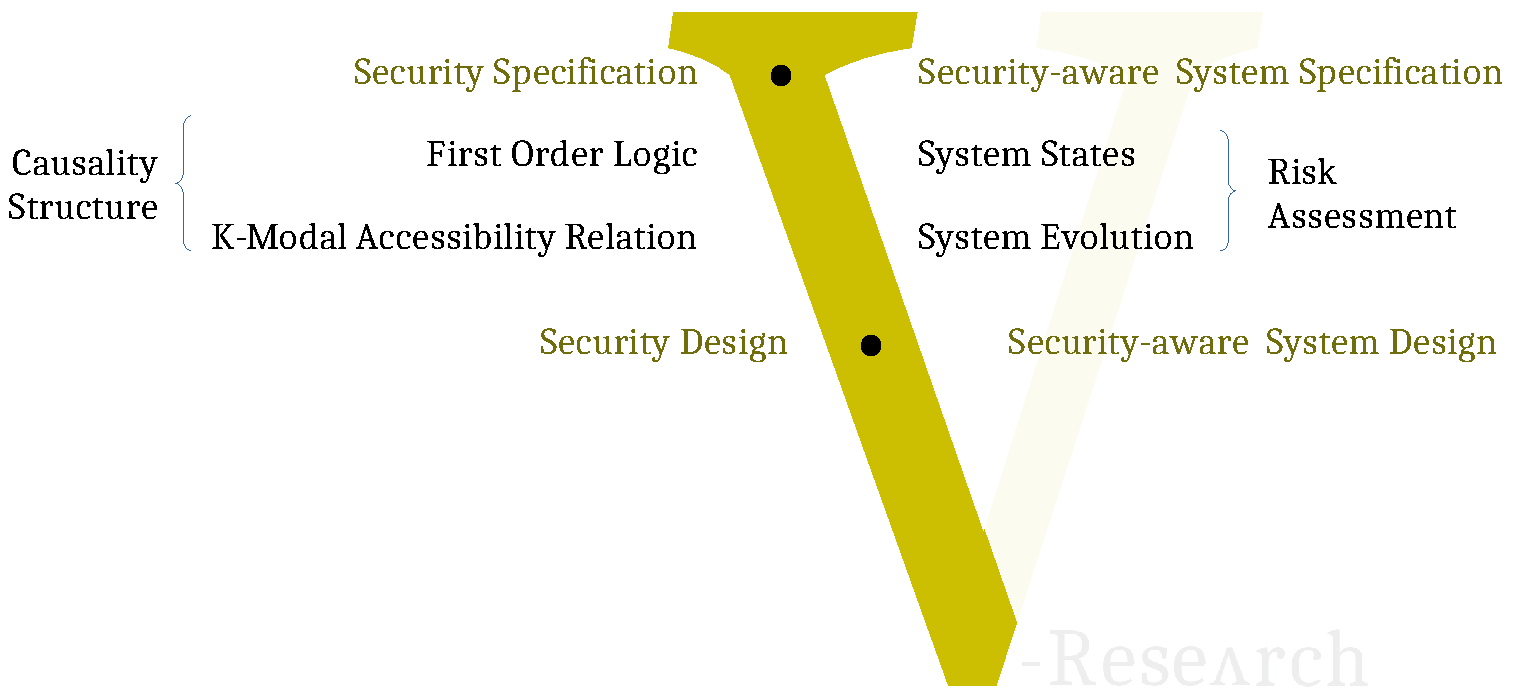
\includegraphics[width=\textwidth]{vmodel.pdf}
	\caption{Cybersecurity Engineering Life-cycle}
	\label{fig:knowledge-belief}
\end{figure}


\subsubsection{Relevant Standards}\label{sec:standards}
\begin{enumerate}[noitemsep]
	\item DO-326A
\end{enumerate}

\section{Honesty and Maliciousness -- A Cybersecurity Theory}\label{sec:theory}
\begin{enumerate}[noitemsep]
	\item cybersecurity as a requirement
	\item vulnerability\label{def:vulnerability}
\end{enumerate}

\section{Prototype and Empirical Tests}\label{sec:prototest}
\subsection{Prototype Implementation}\label{sec:implementation}
\subsection{Empirical Tests}\label{sec:tests}

\section{Conclusion and Related Work}\label{sec:related}

\printbibliography

\begin{appendices}
	\section{RCC3, RCC5, or RCC8}\label{app:rcc}
	\section{Wrong idea 1}
In order to apply consistently the mereotopological structure not just to
reason the agents but also on their evolution, we extend the properties of the
Parthood relation (reflexivity and symmetry) to the modal relation
$\modalrelation$ of the K Modal logic, which in turns defines the causality
principle. This updates the K Modal logic to a B (Brouwer) Modal Logic\autocite{Garson2018modal}.

\begin{definition}{\bf B Modal Logic --}\label{thm:bk-parthood}
	The B Modal Logic (defined, with a slight abuse of notation as
	$\bframe=\langle\possibleworlds,\modalrelation\rangle$) is an extension
	of the K modal logic with the following axioms
	\begin{enumerate}[noitemsep]
		\item[$(\interpretation8)$] $\world\models P\Rightarrow Q$ iff
			$\world\not\models P$ or $\world\models Q$ (logical implication)~\footnote{In
			Definition~\ref{def:modallogic} we didn't specify the
			semantics in the case of the connective $\Rightarrow$
			(i.e. logical implication), so we state it here. Given
			that $P\Rightarrow Q$ is equisatisfiable to
			$\neg(P\wedge \neg Q)$, for any proposition $P$ and
			$Q$, $\world\models P\Rightarrow Q$ is equisatisfiable
			to $\world\models \neg(P\wedge \neg Q)$. If
			$\world\models \neg(P\wedge \neg Q)$ then
			$\world\not\models P\wedge\neg Q$ and then
			$\world\models \neg P$ or $\world\models Q$.}
		\item[$(\interpretation9)$] $\Box P\Rightarrow P$ (which ``claims that whatever is necessary is the case''\autocite{Garson2018modal}), and
		\item[$(\interpretation10)$] $P\Rightarrow\Box\Diamond P$
			(which says that if $P$ is the case, then $P$ is
			necessarily possible\autocite{Garson2018modal})
	\end{enumerate}
\end{definition}

	
\begin{theorem}{\bf Causality, Parthood, and B Modal Logic}\label{thm:bk-parthood}
	\begin{enumerate}[noitemsep]
		\item (Reflexivity) $\bframe\models\Box P\Rightarrow P$ ($\interpretation8$) iff $\modalrelation$ is reflexive
		\item (Symmetry) $\bframe\models P\Rightarrow\Box\Diamond$ ($\interpretation9$) iff $\modalrelation$ is symmetric
		\item (Consistency) $\world\modalrelation\world'$ iff $\connects{\region}{\region'}$
	\end{enumerate}
	whenever $\world$ and $\world'$, and $\region$ and $\region'$ are logically equivalent ($\equiv$).
\end{theorem}
\begin{proof}
	The proof is exhaustive over all possible cases.
	\begin{enumerate}[noitemsep]
		\item(Reflexivity) proven in\autocite{}
		\item(Symmetry) proven in\autocite{}
		\item(Equivalence) \fix{mr}{todo} If
			$\world\modalrelation\world'$ and
			$\world\equiv\region$, then if
			it doesn't hold that $\connects{\region,\region'}$ it
			follows that there is no reflexive and transitive
			relation that correlates $\region$ to $\region'$. Given 
			that Regions are defined as signatures
	\end{enumerate}
\end{proof}

\end{appendices}

\end{document}
